\documentclass{article}
\usepackage{fullpage}
\usepackage{graphicx}


\begin{document}

\title{Spectra and Spectrometers,\\ Vernier Spectrometer,\\ Balmer Spectrum of Hydrogen\\
Modern Physics Laboratory}
\author{Josh Diamond, John Cummings and George Hassel\\
Siena College}
\date{Fall 2020}
\maketitle

\section{Theory}
In this experiment, we display continuous and discrete emission spectra
and explore the use of several types of spectrometers.  Observations
are compared to standard tabulated values and to theoretical
predictions.


\subsection{General features of spectra}
Many light sources in nature produce a mixture of wavelengths.  If
these wavelength components can be separated and displayed
individually, a spectrum results.  Electromagnetic waves that have
been observed cover a tremendous range of wavelength: from radio waves
with wavelengths of hundreds of meters all the way down to gamma rays
with wavelength smaller than the size of an atomic nucleus. In this
experiment, observations are restricted to the relatively tiny visible
portion of the electromagnetic spectrum, for which the wavelengths
cover the range 400-700 nm.

Note:  Common units for visible light wavelengths are the Angstrom
({\AA}), $1 {\rm \AA} = 1 \times 10^{-10} {\rm m}$ and the nanometer (nm), $1 {\rm nm} = 1 \times 10^{-9} {\rm m}$. 

Spectra can be classified as follows:

\begin{enumerate}
\item a continuous spectrum (containing a continuous band of
wavelengths), or 
\item a discrete or line spectrum (containing only certain wavelengths).
\end{enumerate}

One kind of source for a continuous spectrum is any hot, glowing
object--such as the filament of an ordinary incandescent light bulb.
\ A common light source producing a discrete or line spectrum is the
gas-filled electrical discharge tube--e.g. as in a
``neon sign''.

\subsection{Observation of spectra}


Spectra are displayed by passing light from the source through a 
suitable optical device. \ The simplest such device is a prism, which
bends light through angles depending on wavelength. \ Thus, for
example, a single beam of ``white'' light
emerges from a prism as a diverging set of beams which produce the
familiar rainbow spectrum on a screen or the retina of the eye (see
Fig.~\ref{fig:prism})

\begin{figure}
\begin{centering}
 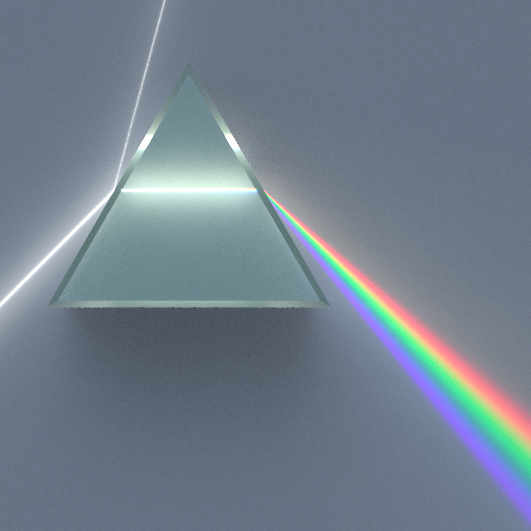
\includegraphics[width=0.75\textwidth]{images/Dispersive_Prism.jpg} 
\caption{White light split into colors by a prism.  The light beam enters the prism from the left, note the reflected beam scattering off to the top of the image.}
\label{fig:prism}
\end{centering}
\end{figure}

The other common device is a diffraction grating--a transparent sheet
with closely-spaced parallel rulings. \ The rulings interrupt the
passage of light, so that the effect is analogous to an opaque plate
with multiple parallel slits. \ If monochromatic light (i.e., light
having a single wavelength) in a collimated beam falls on a grating,
then due to the phenomenon of interference, the light emerging from the
grating is concentrated into several beams, symmetrically deflected
with respect to the original beam direction, as shown in Fig.~\ref{fig:grating}. \ The
beams are labeled by their ``order'', given
by an integer $m$, where $m = 0,1,2,\ldots$.

\begin{figure}
\begin{centering}
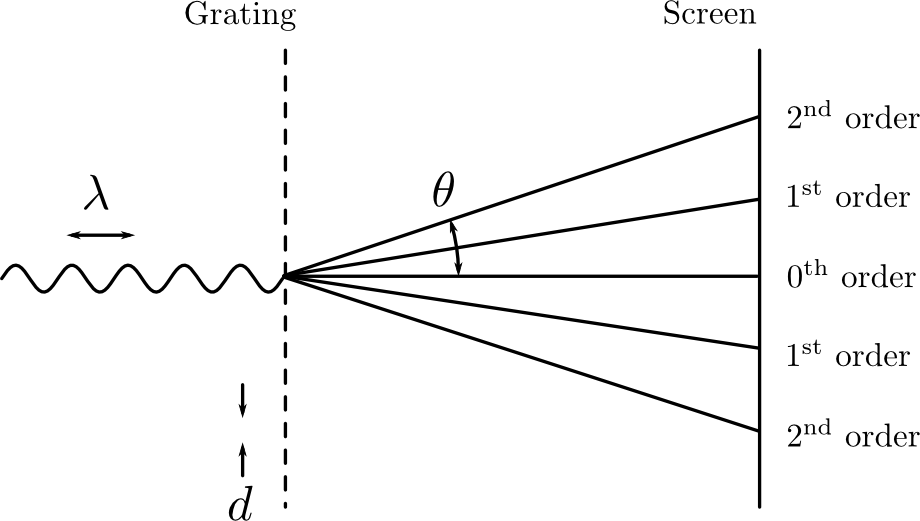
\includegraphics[width=0.75\textwidth]{images/grating-schematic.png} 
\caption{Spectral lines created by a diffraction grating}
\label{fig:grating}
\end{centering}
\end{figure}

One can show theoretically that the mth order beam is deflected by an
angle ${\theta}$, given by the equation: 

\begin{equation}
d \sin \theta = m \lambda
\label{eq:gratingmaxima}
\end{equation}

where ${\lambda}$ is the light wavelength and d is the separation
between adjacent rulings (assumed constant over the entire grating). 


Since the angle ${\theta}$ depends on wavelength, if the incoming light
contains several wavelengths, a complete spectrum will be formed at
each order (except the zeroth). \ Restrictions on angle limit
one's actual observations to the few lowest orders.

\subsection{Theoretical predictions for spectra}
\subsubsection{Balmer spectrum of hydrogen}

The visible spectrum of hydrogen gas is a discrete or line spectrum, and
is one of the simplest observed in nature. \ A look at a photograph of
the spectrum makes it clear that there exists some regularity in the
spectral wavelengths. In 1885, Johann Balmer found an empirical formula
for the visible part of the hydrogen spectrum (the
``Balmer series'', in which the wavelength
${\lambda}$ of the spectral lines is given by:

\begin{equation}
{1 \over \lambda} = R \left( {1 \over 2^2} - {1 \over n^2} \right)
\label{eq:rydberg}
\end{equation}

where $n = 3, 4, 5,\ldots$ and $ R = 1.097 \times 10^7 {\rm m}^{-1}$.

In this equation, each spectral line corresponds to a value of the 
integer $n$.  $R$ is known as the Rydberg constant.  Eq.~\ref{eq:rydberg} provides
an accurate numerical prediction of the Balmer series wavelengths, but
not a scientific understanding of why the visible spectrum of hydrogen
has that behavior. \ Such an understanding first came in 1913 with the
Bohr model of the hydrogen atom, a subject you will take up later in
the course.

\subsubsection{Black body radiation spectrum}
In 1900, Max Planck calculated theoretically the spectrum of light
emitted by an object at a fixed temperature. \ The spectrum is
continuous, and has the simplest form if one assumes that the object is
a ``black body'' i.e. that it is a
perfect absorber of electromagnetic radiation. \ In this case, if the
intensity of emitted light is plotted as a function of the light
wavelength ${\lambda}$, the graph has a single peak. \ The wavelength
${\lambda}_m$ at the peak is related to the absolute
temperature $T$ of the black body by a relation known as
Wien's displacement law:

\begin{equation}
\lambda_m T = 2.898 \times 10^{-3} {\rm m} {\rm K}
\label{eq:wein}
\end{equation}

In Planck's theory, the crucial notion of quantization
was first introduced. \ Planck assumed that the light was emitted in
discrete packets of energy, called quanta or photons. \ The energy E of
a photon was given in terms of a new fundamental constant h as:

\begin{equation}
 E = h\nu = {hc \over \lambda}
\label{eq:plank}
\end{equation}

where $\nu$ and $\lambda$ are the photon frequency and wavelength, and $c$
is the speed of light. \ Planck's constant $h = 6.63 \times 10^{-34} {\rm J} {\rm s}$.

\section{Preliminary Questions}
\begin{enumerate}
\item A diffraction grating has 400 grooves/mm.
\begin{enumerate}
\item Find the spacing between grooves.
\item Calculate the angle at which the first order green mercury
spectral line will occur. \ The mercury green line has wavelength = 546
nm.
\item Calculate the angles at which one would observe all the higher
orders of the green mercury line. \ What is the highest order that can be
observed?
\end{enumerate}

\item Consider Eq.~\ref{eq:rydberg} for the wavelengths of visible spectral lines
emitted by Hydrogen atoms (the Balmer series). \ Which of the allowed
values of the integer n yields the longest wavelength ${\lambda}$?
Explain briefly. \ Now use the equation to compute the three longest
wavelengths in this series. \ For each wavelength, indicate the color
expected of the emitted light.

\item We shall assume in this problem that we can apply the Wien
displacement law to ordinary objects (as opposed to just black
bodies).
\begin{enumerate}
\item Calculate the wavelength at which the maximum amount of light
would be emitted by a person at room temperature. \ In what part of the
electromagnetic spectrum is this wavelength?
\item Repeat part a for molten steel heated to a temperature of 2000
${}^\circ$ C.
\item The wavelength at which peak radiation from the sun is emitted is
approximately 550 nm. \ Determine the surface temperature of the sun.
\end{enumerate}
\end{enumerate}

\section{Equipment}
Incandescent light source, mercury, sodium and hydrogen
vapor lamps, prism, grating, student spectrometer, Vernier spectrometer with optical fiber.
% diode array spectroscopy system.

\section{Notes on Equipment}

\subsection{Student spectrometer}

A schematic top view of the student spectrometer is shown in Fig.~\ref{fig:studentspec}.

\begin{figure}
\begin{centering}
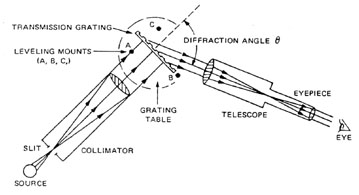
\includegraphics[width=0.75\textwidth]{images/spectrometer-top.jpg} 
\caption{Schematic view of student spectrometer}
\label{fig:studentspec}
\end{centering}
\end{figure}

Light from the source enters the collimator through a narrow
vertically-oriented slit, which then acts like a new source of light.
\ At the other end of the collimator tube is a converging lens, placed
so that its focus is at the slit location. \ Under these conditions
light will emerge from this lens in a collimated beam (parallel rays).
\ If this beam travels unimpeded into the telescope, an observer
looking through the telescope eyepiece will (when the apparatus is
properly adjusted) see a sharp image of the illuminated collimator
slit, which will appear as a bright vertical line.

Figure~\ref{fig:studentspec} shows the spectrometer outfitted with a diffraction grating
mounted on a table at the center of the spectrometer. \ As discussed
above, the effect of the grating is to divide the light into several
beams labeled by their order, \ and within each order (except the
zeroth) to further separate the different wavelengths present. \ When
the telescope is in line with the collimator ($\theta = 0$ in Fig.~\ref{fig:studentspec}),
the zero order (undeflected) beam will be observed--a bright vertical
line with the same color as appears looking directly at the light
source. \ When the telescope is moved away from $\theta=0$, the higher order
beams will appear in succession. If light from the source consists of
several individual wavelengths, then each wavelength produces (in each
order) its own image of the slit. \ These images take the form of
distinct colored lines and are known as ``spectral
lines''. \ We can take quantitative measurements on a
spectral line by moving the telescope so that the line is centered on
the telescope cross hair 
and recording the angular scale reading.

The deflection angle ${\theta}$ entering Eq.~\ref{eq:gratingmaxima} is then determined by
subtraction: 

\begin{equation}
\theta = \left| {\rm(angle\ reading)} - {\rm (zeroth\ order\ angle\ reading)} \right|
\label{eq:calib}
\end{equation}

It is usually most convenient to adjust the spectrometer so that the
zeroth order is at 0 degrees on the angular scale. \ Then the angular
scale reading of the spectral line gives ${\theta}$ directly.

One can also mount a prism on the student spectrometer, in place of a
diffraction grating. \ With the prism there are no multiple orders--
only one spectrum is produced. \ In this experiment we shall use the
prism for qualitative observation only. 

\subsection{Vernier spectrometer}

The Vernier spectrometer, SpectroVis Plus, uses a diffraction grating and CCD detector to measure spectra in the range of 380-950 nm.   The unit interfaces with LoggerPro to collect and record data. We will use the optical fiber accessory for the measurements in this activity.

\begin{figure}
\begin{centering}
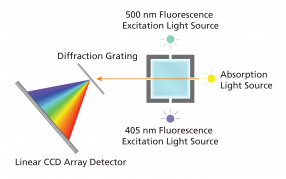
\includegraphics[width=4.4862in,height=2.972in]{images/SpectroVisDiagram.png} 
\caption{SpectroVis diagram}
\label{fig:spectrovisdiagram}
\end{centering}
\end{figure}



%\subsection{Constant deviation prism spectrometer}

%The constant deviation prism spectrometer is a precision instrument
%which gives a direct reading of the wavelength of spectral lines. \ The
%geometry of the prism and a typical light ray path is shown in Fig.~\ref{fig:constdevprism}

%\begin{figure}
%\begin{centering}
%\includegraphics[width=4.4862in,height=2.972in]{spec-img4.png} 
%\caption{Constant deviation prism geometry}
%\label{fig:constdevprism}
%\end{centering}
%\end{figure}

%This prism is so constructed that if a monochromatic beam is incident on
%face $AB$ of the prism at an angle $I$ such that $\sin(I) = n/2$ , then the
%outgoing beam emerging from face $BC$ will be traveling in a direction
%exactly 90 degrees from the incoming beam. \ Here, $n$ is the index of
%refraction of the prism glass for the light wavelength present. \ In
%the notation of Fig.~\ref{fig:constdevprism} the perpendicularity of the two beams implies
%that the angles $I$ and $E$ are equal.

%In the constant deviation spectrometer, the collimator and telescope are
%permanently mounted perpendicular to each other. In order to observe a
%particular spectral line in the telescope, the prism must be rotated
%(thus varying $I$) until the condition $\sin(I) = n/2$ is met for light of
%that wavelength. \ Different wavelengths have different
%$n$'s and hence will appear for different values of $I$.
%\ The dial which rotates the prism also turns a scale constructed to
%give directly the wavelength of the spectral line being viewed.

%A button on the top of the spectrometer allows one to fix the position
%of the adjustable cross hair exactly on a spectral line of well-known
%wavelength (e.g. the bright yellow line of sodium). This is the only
%calibration of the instrument needed prior to use. \ This process is
%described below in the Procedure section.

%\subsection{Diode array spectroscopy system}
%
%This device uses a grating as its wavelength-sensitive element. \ After
%reflecting from a the grating (contained in a monochrometer), the light
%strikes a diode array detector consisting of 1024 light-sensitive
%diodes, each about 25 microns wide. The entire array is approximately
%$1000 \times .025 {\rm mm} = 25 {\rm mm} \approx 1$ inch in width. \ The light coming
%from the grating is deflected by an angle depending on its wavelength,
%and hence the different wavelengths will fall on different parts of the
%diode array detector. \ The electronics and computer software supplied
%with the array permit the resulting output to be a graph of light
%intensity vs wavelength over a range of wavelengths that can be set by
%the experimenter.

\section{Procedure}

Note: \ Answer all questions in the procedure section during the
laboratory period and include as part of your data. 

\subsection{Adjustment of the student spectrometer}
\begin{enumerate}
\item Place the spectrometer on a flat level surface.
\item Point the telescope so that it is not in line with the collimator.
Move the eyepiece so that the cross hairs are in focus.
\item Look through the telescope at a distant object (out a window or
across the room) and move the entire front tube of the telescope until
the object is in focus. \ The sharpness of the image of the cross hairs
should not be affected by this step.
\item Align the telescope and collimator. \ Open the collimator slit to
its maximum size. \ Loosen the screw holding the sleeve at the slit end
of the  collimator tube. Move this tube until the image of the slit as
viewed  through the telescope is in focus and is aligned vertically.
(During this adjustment, the sleeve should be held in position so that
its ``V point'' fits into the V-shaped notch
on the collimator mounting.)  Now tighten the sleeve screw. The
spectrometer should now be satisfactorily adjusted optically.
\item Narrow the slit and align the telescope so that the slit appears
accurately centered on the cross-hairs.  Check the angular scale
reading.
If it is not already zero, adjust the scale table so that the reading is
zero.  Make sure the telescope slit stays aligned with the cross-hairs
in this process (the telescope can actually be locked in place
temporarily for this purpose). Consult the instructor for assistance if
needed.
\item If the slit image appears too high or too low in the telescope
field of view, the telescope may be tilted up or down by use of the
adjustment screws on its mount.  Small adjustments should be
sufficient.
\end{enumerate}

\subsection{Student prism spectrometer}
Note: These observations with the prism spectrometer are
qualitative--no angular scale measurements needed.

\begin{enumerate}
\item Place a prism on the central table of the spectrometer and align
the prism so that light from the collimator will enter one of its faces
as illustrated in Fig.~\ref{fig:prism}.  Note that the light should not strike the
prism perpendicular to its face. Use the clamp to hold the prism in
place; also adjust the table to the proper height if needed. 


From what face would you expect light to exit the prism? \ In what
general direction? (Look at Fig.~\ref{fig:prism} and recall how light bends when it
travels from air into glass and then from glass back into air.). Now
align the telescope to be able to view light exiting from the prism.

\item Place an incandescent light source in front of the collimator.
Note: this light will likely be bright, so be sure the collimator slit
is narrowed! Observe the spectrum of the incandescent source through
the telescope.   (You will need to move the telescope to find the
spectrum and to see the various colors.)  Describe briefly and sketch.
 Which color is deflected the most by the prism from the original
light beam direction?  Which color is deflected the least? 

\item Observe the spectra of a sodium lamp and a mercury vapor lamp (or
discharge tube). How do these spectra differ from that of the
incandescent source? In each case, make a sketch of the observed
spectral lines and indicate the color of each line.
\end{enumerate}

\subsection{Student grating spectrometer}
Note:  Record all angular position readings to the nearest tenth of a
degree.  It is not necessary to use the vernier scale for measurements
in this experiment.

\begin{enumerate}
\item Replace the prism clamp with the grating holder and mount a grating
on the spectrometer table as shown in Fig.~\ref{fig:studentspec}.  Observe the
incandescent light spectrum.  Starting from the zero order position,
move the telescope gradually to the maximum meaningful value of
deflection angle ${\theta}$ (what is this value?).  How many orders of
the spectrum are visible? 

For the first order spectrum, record the deflection angle ${\theta}$ of
the extreme edges of the spectrum (i.e., the extreme red and extreme
violet).

Important note: Check your angular scale reading for the zeroth order.
 Is it zero?  If you have not zeroed the angular scale as described
in the procedure above, the zeroth order angle must also be recorded,
and then the deflection angle ${\theta}$  for non-zero orders obtained
using Eq.~\ref{eq:calib}. This correction will also be needed in steps 2 and 3
below.

\item Observe the spectrum of a sodium lamp.  How many orders are
visible? Record the deflection angle ${\theta}$ at which the bright
yellow line appears, for all orders you can see.

\item Now use the mercury vapor lamp or discharge tube.  Note: Spectral
lines from this source tend to be dimmer, so your eyes should be well
dark-adapted.  Also, it helps to widen the collimator slit somewhat.

Starting with the first order, carefully list all the spectral lines you
can see as the angle ${\theta}$ is increased from zero.  Record the
angular position of each line. Tabulate your results, including the
color, order and deflection angle ${\theta}$ of each line.  Also give
an indication of the brightness of each line (e.g. strong=s, medium=m,
weak=w). 

\item Note in your data table for the previous step any instances in
which a higher order line of one color appeared before a lower order
line of a different color (i.e., the higher-order line had a smaller
deflection angle  than the lower order line).  This is called
``overlapping of orders''.

\item Record the number of rulings per unit length for the grating.
\end{enumerate}

\subsection{Vernier Spectrometer}

\begin{enumerate}
\item Set up the spectrograph:
\begin{enumerate}
\item Connect the SpectroVis Plus directly to the laptop using the USB cable (not through the LabPro or other interface).   Place the optical fiber in the square opening in the spectrometer.  
\item Start LoggerPro.  Choose Experiment $\rightarrow$ Calibrate and follow the instructions to calibrate the spectrograph.
\item Choose Experiment $\rightarrow$ Change Units to change to an Intensity graph
\end{enumerate}
\item Place the H emission tube in the power supply and turn it on.  Bring the optical fiber near but not touching the tube, and record the spectrum by pressing the Collect (green "Play" button)
\item Click the red "Stop" button when you obtain a suitable spectrum.  Use the Examine button to identify the wavelengths of the discrete lines.
\item Repeat the previous steps for an Hg emission tube.  Turn off the power supply before changing tubes and be aware that the tube may be hot.
\item Repeat the previous steps for a mystery tube.  Turn off the power supply before changing tubes and be aware that the tube may be hot.
\item Record a spectrum for the fluorescent lights in the ceiling.   
\end{enumerate}

%\subsection{Constant Deviation Prism Spectrometer}
%\begin{enumerate}
%\item Adjustment and Calibration of Constant Deviation Prism
%Spectrometer
%\begin{enumerate}
%\item Open collimator slit to maximum width.
%\item Slide collimator slit ``V'' mask to give maximum slit height.
%\item Place sodium lamp at collimator slit.
%\item  Adjust wavelength dial to 580 nm.  Press down on spring-loaded
%button located on the top of the spectrometer.  While holding the
%button down, slowly turn the wavelength dial toward 600 nm.  The
%button will drop downward and lock the dial at about 590 nm.  This is
%the calibration point for the sodium yellow line.  Do not move the
%wavelength dial until calibration is complete.
%\item Look through the telescope.  A bright yellow rectangle should
%appear.  If it does not appear, try pulling the two metal strips on
%each side of the telescope piece all the way out.  The rectangle is
%the``spectral line'' for the sodium
%yellow light.  It is actually an image of the illuminated slit on the
%collimator.  Adjust the telescope eyepiece so that the spectral line
%is in sharp focus.  A pair of cross hairs in the shape of an X should
%be visible and should also be in focus.
%\item Turn the screw to the right of the telescope eyepiece.  Notice
%that this moves the cross hairs to the right or left.  Move the cross
%hairs so that their intersection point is at the center of the spectral
%line.
%\item Narrow the spectral line image with the slit edge adjustment
%controls--the flat metal strips on each side of the telescope
%eyepiece--while keeping the cross hair intersection centered.
%\end{enumerate}

%The constant deviation prism spectrometer is now calibrated and ready to
%provide a direct readout of the spectrum wavelengths of other light
%sources.

%\item With the mercury vapor source in place, observe and record the
%wavelengths of all visible spectral lines.

%\item Repeat step 2 for the hydrogen discharge tube.

%\end{enumerate}

%\subsection{Diode Array Spectroscopy System}
%Note:  Refer to the Appendix: Instructions for Diode Array Spectroscopy
%System for specific steps in the operation of the diode array
%apparatus.  The monochrometer dial setting and computer parameters
%must be consistent in order to get meaningful readings.  Ask your
%instructor to check these settings before starting to record data.
%
%\begin{enumerate}
%\item Set the computer parameters and the monochrometer for incandescent
%lamp source (continuous spectrum), as explained in the Appendix.  Note: The same
%settings will also be used for Step 2.
%
%Set the voltage of the variac powering the light bulb to 60 volts.
% Note and record the visual appearance of the filament (color and
%brightness).
%
%Now take a spectrum of the light emitted by the filament with the diode
%array apparatus. \ From the plot on the computer screen, use the cursor
%commands to determine the wavelength at the maximum (peak) intensity
%and record the result. \ Print the spectrum. (Note: the printed
%spectrum will not include the numerical value of the wavelength at peak
%intensity, so you must record this wavelength by hand.)}
%
%
%\bigskip
%
%{\selectlanguage{english}
%2. \ Repeat Step 1 for variac voltages 90 and 120 volts. \ In
%qualitative terms, how does the wavelength at peak intensity vary as a
%function of the temperature of the filament? }
%
%
%\bigskip
%
%{\selectlanguage{english}
%3. \ Now set the computer parameters and the monochrometer for gas
%discharge tube source (discrete spectrum), as explained in the
%Appendix. \ You will take two spectra, one for the lower wavelength
%range of the visible spectrum, and one for the upper range. \ \ }
%
%
%\bigskip
%
%{\selectlanguage{english}
%Observe the spectrum of mercury vapor in the lower and in the upper
%visible wavelength ranges. \ Record the peak wavelength of each of the
%observed spectral lines. \ \ Print the two spectra.}
%
%
%\bigskip
%
%{\selectlanguage{english}
%Observe the spectrum of hydrogen gas in the lower and in the upper
%visible wavelength ranges. \ Record the peak wavelength of each of the
%observed spectral lines. \ Print the two spectra.}
%
%
%\bigskip
%
%
%\bigskip
%
%
%\bigskip
%
%
%\bigskip
%
%
%\bigskip
%
%\clearpage{\selectlanguage{english}


\section{Analysis}

\begin{enumerate}
\item Use the data of step 5.3.1 of the procedure to calculate the
wavelengths of the limits of the incandescent light spectrum.  These
will be the limits of your vision.

\item Based on the values of ${\theta}$ measured with the student grating
spectrometer, use Eq.~\ref{eq:gratingmaxima} to compute the wavelength of the bright
yellow line of the sodium lamp spectrum.  If you observed more than
one order, find the wavelength for each order and compute the average.
 Compare with the value tabulated below.

\begin{table}
\begin{tabular}{ l | l | l | l | l}
  Sodium & Mercury & Helium & Cadmium & Hydrogen \\
\hline
5889.95 (s) & 4046.56 (m) & 4387.93 (w) & 4678.16 (m) & 4101.47 (w) \\
5895.92 (m) & 4077.81 (m) & 4437.55 (w) & 4799.92 (s) &  4340.46 (w)\\
		 & 4358.35 (s) & 4471.48 (s) & 5085.82 (s) & 4861.33 (m) \\
		 & 4916.04 (w) & 4713.14 (m) & 6438.47 (s) &  6562.82 (s)\\
		 & 5460.74 (s) & 4921.93 (m) &  & \\
		 & 5769.59 (s) & 5015.67 (s) &  & \\
		 & 5790.65 (s) & 5047.74 (w) &  & \\
		 & 6152    (m) & 5875.62 (s) &  & \\
		 & 6910    (m) & 6678.15 (s) &  & \\
\end{tabular}
\caption{Wavelengths of selected spectral lines [\AA].  s: strong, m: medium, w: weak}
\end{table}


\item Use the measured values of the angle ${\theta}$ to calculate the
wavelength of the lines in the mercury vapor spectrum observed with the
student grating spectrometer.  Each line should be identified by its
color and order. If a line was observed in more than one order,
calculate the average wavelength for that color.  Compare these
calculated average wavelengths to the wavelengths measured for the same
lines with the Vernier spectrometer.
% and with the diode array system.
Also compare to the standard wavelength values
tabulated above.  Try to account for any discrepancies.

\item In preliminary question 2, you calculated predicted wavelengths of
the visible spectrum of hydrogen (from Balmer's
empirical formula--Eq.~\ref{eq:rydberg}) and noted the corresponding colors.
Compare the predicted hydrogen wavelengths to those you observed
using the Vernier spectrometer.  For each predicted
wavelength, identify the observed spectral line (if any) whose
wavelength appears to approximate the predicted value.  Indicate the
value of the integer $n$ (in the Balmer series formula (Eq.~\ref{eq:rydberg})) for each
spectral line so identified.

\item Use Table 1 and your measured spectrum to identify the gas in the mystery tube.   

\item Use Table 1 and your previous spectra to determine if any elemental gases are in the fluorescent light bulb. 

\end{enumerate}

%\bigskip
%
%{\selectlanguage{english}
%5. \ Explain qualitatively in terms of the photon model of light your
%visual observations of the continuous spectrum emitted by the hot
%filament and your measurements using the diode array system. \ Consider
%in particular the behavior of the various quantities observed as a
%function of the filament temperature. }
%
%
%\bigskip
%
%{\selectlanguage{english}
%Also, use Eq. (3) to calculate the filament temperature at each of the
%three variac voltages. \ \ \ }
%
%
%\bigskip
%
%
%\bigskip
%
%
%\bigskip
%
%{\centering\selectlanguage{english}\bfseries
%APPENDIX: INSTRUCTIONS FOR 
%\par}
%
%{\centering\selectlanguage{english}\bfseries
%DIODE ARRAY SPECTROSCOPY SYSTEM
%\par}
%
%
%\bigskip
%
%
%\bigskip
%
%{\selectlanguage{english}\bfseries
%1. \ Opening spectroscopy system software.}
%
%{\selectlanguage{english}
%Double-click on the Instaspec icon on the desktop.}
%
%
%\bigskip
%
%{\selectlanguage{english}
%\textbf{2. \ Checking user-defined spectrograph values.}}
%
%{\selectlanguage{english}
%From the Hardware menu select Setup Spectrograph. \ In this window, the
%choices should }
%
%{\selectlanguage{english}
%already be correctly set at the following values, which correspond to
%the 1/4 m monochrometer.}
%
%{\selectlanguage{english}
%{}-{}-Spectrograph: UserDefined}
%
%{\selectlanguage{english}
%{}-{}-Focal length (meters): 0.25}
%
%{\selectlanguage{english}
%{}-{}-Angular deviation (degrees): 13.94}
%
%{\selectlanguage{english}
%{}-{}-Focal plane tilt (degrees): 3.626}
%
%
%\bigskip
%
%{\selectlanguage{english}
%If any of the settings are different from the above, then correct them.
%\ Then click on OK.}
%
%
%\bigskip
%
%{\selectlanguage{english}\bfseries
%3. Calibrating spectrograph. }
%
%{\selectlanguage{english}
%From the Calibrate menu, select X Calibration by Spectrograph. \ In that
%window, the following settings should be entered:}
%
%
%\bigskip
%
%{\selectlanguage{english}
%{}-{}-X-axis label: Wavelength}
%
%{\selectlanguage{english}
%{}-{}-Units: nm}
%
%{\selectlanguage{english}
%{}-{}-Center Wavelength: }
%
%{\selectlanguage{english}
%\ \ \ \ \ \ \ \ {}- Incandescent lamp source (continuous spectrum): 750
%nm }
%
%{\selectlanguage{english}
%\ \ \ \ \ \ \ \ {}-Gas discharge tube source (discrete spectrum): \ 480
%nm for lower wavelength range; }
%
%{\selectlanguage{english}
%600 nm for upper wavelength range \ }
%
%{\selectlanguage{english}
%{}-{}-Grating (lines/mm): 400}
%
%{\selectlanguage{english}
%{}-{}-Offset: Default is 0. \ May be shifted later to improve
%calibration. \ See Step 10 below.}
%
%
%\bigskip
%
%{\selectlanguage{english}
%After entering settings, click on Calibrate and then close window.}
%
%
%\bigskip
%
%{\selectlanguage{english}
%\textbf{4. \ Selecting acquisition mode.}}
%
%{\selectlanguage{english}
%From the Acquisition menu, select Setup Acquisition. \ The Acquisition
%mode should be }
%
%{\selectlanguage{english}
%Single Scan, and the Trigger Mode should be Internal. \ The default
%values of the numerical parameters are normally adequate for this
%experiment.}
%
%
%\bigskip
%
%{\selectlanguage{english}
%\textbf{5. \ Selecting data type. }}
%
%{\selectlanguage{english}
%From the Acquisition menu, select Setup Data Type. \ \ Choose Counts [Bg
%corrected]. }
%
%
%\bigskip
%
%
%\bigskip
%
%{\selectlanguage{english}
%\textbf{6. Calibrating the monochrometer.}}
%
%{\selectlanguage{english}
%{}-{}-For the incandescent lamp source, set wavelength dial to 250.0
%\ [250 = (1/3)(750)]}
%
%{\selectlanguage{english}
%{}-{}-For a gas discharge tube source, set wavelength dial to 160.0 [160
%= (1/3)(480)] for lower wavelength range. Set dial to 200.0 [200 =
%(1/3)(600)] for upper wavelength range.}
%
%
%\bigskip
%
%{\selectlanguage{english}
%\textbf{7. \ Taking a background scan.}}
%
%{\selectlanguage{english}
%Cover the end of the fiber optic input light cable. \ From Acquisition
%menu, click on Take }
%
%{\selectlanguage{english}
%Background. \ A graph should appear with a noisy, featureless spectrum.
%\ This is due to background electronic noise in the diode array
%detector. \ By using the data type Counts [Bg corrected], this
%background spectrum will be automatically subtracted from the overall
%number of counts, so that the data displayed is (approximately) just
%the spectrum due to the light source being studied. }
%
%
%\bigskip
%
%{\selectlanguage{english}
%\textbf{8. \ Taking a spectrum; cursor commands. }}
%
%{\selectlanguage{english}
%{}-{}-Uncover the end of the fiber optic cable. \ Move the light source
%into position in front of the end of the cable. \ From the Acquisition
%menu, click on Take Signal (or click on the green button in the
%toolbar). \ A graph will appear with the spectrum of the light source.}
%
%
%\bigskip
%
%{\selectlanguage{english}
%{}-{}-You move the cursor with the right and left arrow keys. \ Reading
%left to right below the graph, the first two numbers are the wavelength
%(x coordinate) and the number of counts (y coordinate) of the point
%where the cursor is located. \ Try moving the cursor and watching the
%numbers change. \ Note: The number of counts is proportional to the
%light intensity at that wavelength.}
%
%
%\bigskip
%
%{\selectlanguage{english}
%{}-{}-In this experiment you will need the wavelengths at the peak (or
%peaks) in the various spectra observed. \ Ctrl/right arrow moves the
%cursor to the next peak on the right.\textbf{ \ }Ctrl/left arrow moves
%the cursor to the next peak on the left. \ The cursor will not move if
%there are no peaks in the direction specified.}
%
%
%\bigskip
%
%{\selectlanguage{english}
%\textbf{9. \ Printing a spectrum. }}
%
%{\selectlanguage{english}
%To print the spectrum on the screen, select Print from the file menu.}
%
%
%\bigskip
%
%{\selectlanguage{english}
%\textbf{10. \ Calibrating the offset.}}
%
%{\selectlanguage{english}
%To calibrate the offset, take a spectrum of a sodium lamp. \ The
%monochrometer dial should be set at 200.0 (see step 6). \ \ The main
%peak should appear at a wavelength of 589.3 nm. \ If the wavelength at
%the peak differs from that value, then adjust the offset (see step 3
%above) to shift the peak to the correct value. \ Take another sodium
%spectrum to check its position. \ Repeat the offset adjustment until
%the sodium peak is correctly positioned. \ }
%
%
%\bigskip
%
%{\selectlanguage{english}
%Note: the offset is calibrated in pixels, not nm, so you will have to
%determine by trial and error what numerical value of the offset will
%yield the correct wavelength for the peak.}
%
%

\section{References}

\begin{itemize}
\item Thornton and Rex, Modern Physics $3^{\rm rd}$ edition, pp. 92-103
\item Tipler and Llewellyn, Modern Physics $5^{\rm th}$ edition, pp. 119-121, 147-150.
\item Vernier SpectroVis Plus Spectrophotometer Manual (SVIS-PL)
\end{itemize}

\end{document}
